\documentclass[conference]{IEEEtran}
\IEEEoverridecommandlockouts

% === CẤU HÌNH FONT & NGÔN NGỮ ===
\usepackage[utf8]{inputenc}
\usepackage[T5]{fontenc}
\usepackage{lmodern}
\usepackage[vietnamese]{babel}

\usepackage{cite}
\usepackage{amsmath,amssymb,amsfonts}
\usepackage{algorithmic}
\usepackage{graphicx}
\graphicspath{{../results/figures/}{results/figures/}{./}}
\usepackage{textcomp}
\usepackage{xcolor}
\usepackage{booktabs}
\usepackage{tabularx}
\usepackage{microtype}
\usepackage{hyperref}

\hypersetup{
    colorlinks=true,
    linkcolor=black,
    citecolor=black,
    urlcolor=blue
}

\begin{document}

% =========================================================================
% TIÊU ĐỀ VÀ TÁC GIẢ (CĂN CHỈNH GỌN GÀNG, 2 HÀNG CÂN ĐỐI, KHÔNG TRÀN LỀ)
% =========================================================================

\title{\LARGE\bfseries Sắp xếp khóa số nguyên quy mô lớn:\\thuật toán giáo trình và pdqsort\thanks{Báo cáo đồ án môn học CSD201 -- Cấu trúc dữ liệu và Giải thuật (Fall 2026, Lớp SE20C, Mã đề: 261014). Ngành Kỹ thuật Phần mềm (Software Engineering), Đại học FPT.}
}

\author{
\IEEEauthorblockN{Nguyễn Thành Danh, Võ Xuân Long, Phan Văn Bảo\\Nguyễn Nhật Tường Vy, Trần Hoàng Thịnh, Nguyễn Đồng Tấn Phước}
\IEEEauthorblockA{Ngành Kỹ thuật Phần mềm (Software Engineering), Trường Đại học FPT\\
Lớp: SE20C -- Nhóm 6 -- Đề tài 1: Sắp xếp khóa số nguyên quy mô lớn và pdqsort}
}

\maketitle

% =========================================================================
% TÓM TẮT & TỪ KHÓA BẰNG TIẾNG VIỆT
% =========================================================================

\begin{abstract}
Sắp xếp mảng khóa số nguyên 32-bit không âm quy mô lớn là tác vụ nền tảng trong các hệ thống database và đối soát giao dịch tài chính. Trong khi các ngôn ngữ hiện đại như Go và Rust đã chuẩn hóa sang thuật toán lai thích ứng Pattern-Defeating Quicksort (pdqsort), giáo trình đại học chuẩn vẫn tập trung vào các giải thuật kinh điển: Quick Sort, Merge Sort, Heap Sort và Radix Sort. Nghiên cứu này triển khai thực nghiệm có kiểm soát chặt chẽ trên 5 phân phối dữ liệu ($D_1 \to D_5$) với quy mô mở rộng từ $10^5$ đến $2\times 10^7$ phần tử. Các chỉ số đo gồm runtime, đỉnh bộ nhớ phụ heap, số phép so sánh khóa, số thao tác truy cập mảng và độ sâu call stack trong tiến trình JVM độc lập. Đồng thời, nghiên cứu thực hiện ablation study bóc tách định lượng đóng góp của cơ chế nhận diện dữ liệu presorted (Cơ chế A) và gom khóa trùng (Cơ chế B) trong pdqsort, kết hợp kiểm thử đối kháng bằng hoán vị killer adversary của Musser. Kết quả thực nghiệm khẳng định LSD Radix Sort đạt throughput cao nhất với thời gian tiệm cận $O(N)$ ổn định trên mọi phân phối. Heap Sort bảo đảm nghiêm ngặt bộ nhớ phụ $O(1)$ in-place nhưng chịu suy giảm hiệu năng do cache miss. pdqsort chứng minh sự vượt trội toàn diện khi đạt tốc độ $O(N)$ trên dữ liệu presorted, loại bỏ hoàn toàn suy thoái khi trùng lặp khóa và triệt tiêu nguy cơ $O(N^2)$ nhờ fallback Introsort, cung cấp tiêu chí lựa chọn giải thuật rõ ràng cho các hệ thống xử lý dữ liệu lớn.
\end{abstract}

\begin{IEEEkeywords}
Integer sorting, Quick Sort, Radix Sort, Heap Sort, pdqsort, algorithm benchmarking, empirical evaluation.
\end{IEEEkeywords}

% =========================================================================
% MỤC I: GIỚI THIỆU
% =========================================================================
\section{Giới thiệu}
Trong các hệ thống xử lý giao dịch tài chính và đối soát dữ liệu ngân hàng, việc sắp xếp các lô dữ liệu gồm hàng chục triệu khóa số nguyên 32-bit ($0 \le x \le 2^{31}-1$) là tác vụ diễn ra thường nhật. Trong thực tế, dữ liệu hiếm khi hoàn toàn ngẫu nhiên: nhiều lô dữ liệu gần như đã có thứ tự theo mốc thời gian, hoặc chứa mật độ phần tử trùng lặp rất lớn.

Giáo trình Cấu trúc dữ liệu và Giải thuật chuẩn (CLO6) chủ yếu trang bị bốn thuật toán kinh điển: Quick Sort, Merge Sort, Heap Sort và Radix Sort. Ngược lại, nhiều ngôn ngữ hiện đại đã chuẩn hóa sang pdqsort do Orson Peters đề xuất \cite{peters2021pdqsort}. pdqsort kết hợp tốc độ trung bình vượt trội của Quick Sort với khả năng tự nhận diện dữ liệu có thứ tự, gom khóa trùng và cơ chế Introsort fallback để bảo đảm nghiêm ngặt cận trên $O(N \log N)$.

Để cung cấp cơ sở khoa học định lượng cho việc lựa chọn giải thuật trong các hệ thống thực tế, nghiên cứu này giải quyết ba câu hỏi nghiên cứu cốt lõi:
\begin{itemize}
    \item \textbf{RQ1 (Quy mô dữ liệu):} Bốn thuật toán giáo trình khác nhau như thế nào về runtime, đỉnh bộ nhớ phụ và số thao tác cơ bản khi quy mô $N$ tăng từ $10^5$ đến $2\times 10^7$ trên phân phối ngẫu nhiên $D_1$?
    \item \textbf{RQ2 (Đặc trưng dữ liệu):} Mức độ có thứ tự ($D_1 \to D_4$) và mật độ trùng khóa ($D_5$) làm thay đổi thứ hạng tương đối của bốn thuật toán giáo trình như thế nào tại $N = 10^7$?
    \item \textbf{RQ3 (Đóng góp của pdqsort):} pdqsort cải thiện bao nhiêu so với Quick Sort giáo trình trên các dạng dữ liệu của RQ2, và mỗi cơ chế cốt lõi gồm Cơ chế A (nhận diện presorted) và Cơ chế B (gom khóa trùng) đóng góp bao nhiêu thông qua ablation study (\texttt{noA}, \texttt{noB})?
\end{itemize}

% =========================================================================
% MỤC II: CƠ SỞ LÝ THUYẾT
% =========================================================================
\section{Cơ sở lý thuyết}

\subsection{Các thuật toán dựa trên so sánh khóa}
\textbf{Quick Sort} do Hoare đề xuất \cite{hoare1962quicksort} áp dụng kỹ thuật chia để trị. Với phân hoạch Hoare hai con trỏ và chọn chốt median-of-three, thuật toán có độ phức tạp trung bình $O(N \log N)$ nhưng vẫn đối mặt với nguy cơ thoái hóa $O(N^2)$ và tràn call stack (\texttt{StackOverflowError}) khi gặp các mẫu dữ liệu killer adversary \cite{musser1997introsort, mcilroy1999killer}.

\textbf{Merge Sort} bảo đảm thời gian $O(N \log N)$ trong mọi trường hợp và bảo toàn tính stable \cite{sedgewick2011algorithms}. Tuy nhiên, nhược điểm chí mạng là đòi hỏi không gian mảng phụ $O(N)$, tạo áp lực lớn lên bộ nhớ heap và bộ nhớ cache.

\textbf{Heap Sort} do Williams đề xuất \cite{williams1964heapsort} sử dụng Max-Heap in-place, bảo đảm thời gian worst-case $O(N \log N)$ và bộ nhớ phụ nghiêm ngặt $O(1)$. Song, do truy cập nhảy bước xa trên cây nhị phân ($2i+1, 2i+2$), Heap Sort chịu tổn thất nặng nề về tính cục bộ bộ nhớ cache locality.

\subsection{Thuật toán phân phối phi so sánh}
\textbf{Radix Sort} (LSD) \cite{sedgewick2011algorithms} bóc tách khóa nguyên theo từng nhóm bit (cơ số 256, 8-bit/lượt). Thuật toán không so sánh giá trị khóa mà phân phối dựa trên Counting Sort, đạt độ phức tạp lý thuyết $O(k \cdot N)$ với $k=4$ lượt cho số nguyên 32-bit.

\subsection{Pattern-Defeating Quicksort (pdqsort)}
pdqsort \cite{peters2021pdqsort} khắc phục triệt để các hạn chế của Quick Sort bằng các kỹ thuật:
1) Ngưỡng cơ sở chuyển sang Insertion Sort khi đoạn con $N < 24$.
2) Chọn pivot thích nghi với Tukey's Ninther \cite{bentley1993engineering} khi $N > 128$.
3) \textbf{Cơ chế A:} Thử partial insertion sort trên hai nửa nếu phân hoạch cân bằng và không có hoán đổi, đạt độ phức tạp $O(N)$ trên dữ liệu tăng dần.
4) \textbf{Cơ chế B:} Gom các khóa bằng pivot sang trái khi pivot bằng phần tử liền trước, loại trừ suy thoái trên mảng trùng lặp.
5) Chống suy thoái (Introsort limit): Đếm số lần phân hoạch lệch; nếu vượt $\lfloor \log_2 N \rfloor$ thì lập tức chuyển sang Heap Sort trên đoạn đang xét.

% =========================================================================
% MỤC III: PHƯƠNG PHÁP CÀI ĐẶT
% =========================================================================
\section{Phương pháp cài đặt}

Mọi thuật toán được hiện thực bằng Java 17 trên mảng thuần nguyên bản \texttt{int[]}, không dùng kiểu bao gói \texttt{Integer[]} hay \texttt{Comparator}.

\subsection{Cài đặt bốn thuật toán giáo trình}
\textbf{Quick Sort (Cặp 1):} Hiện thực chuẩn phân hoạch Hoare hai đầu: hai con trỏ $i, j$ chạy hội tụ từ hai phía và dừng lại ngay khi gặp khóa bằng pivot ($a[i] \ge \text{pivot}$ và $a[j] \le \text{pivot}$). Pivot được lựa chọn bằng hàm \texttt{medianOfThree(lo, mid, hi)}. Thuật toán đệ quy cả hai phía, không dùng phân hoạch Lomuto.

\textbf{Merge Sort (Cặp 1):} Hiện thực Top-Down đệ quy. Để triệt tiêu chi phí cấp phát lặp lại và giảm áp lực lên Garbage Collector (GC), thuật toán chỉ cấp phát duy nhất một lần mảng phụ kích thước $N$ (\texttt{int[] aux = new int[N]}) tại hàm gốc ban đầu và truyền xuyên suốt cây đệ quy. Điểm chia đôi dùng phép dịch bit không dấu \texttt{mid = lo + ((hi - lo) >>> 1)} để chống tràn số nguyên. Quá trình trộn giữ nghiêm ngặt tính chất stable và không thêm nhánh bỏ qua trộn.

\textbf{Heap Sort (Cặp 2):} Hiện thực Max-Heap in-place bằng phương pháp dựng heap bottom-up từ chỉ số $(n/2 - 1)$ xuống $0$. Mô-đun cung cấp hàm \texttt{public static void sortRange(int[] a, int lo, int hi)} hỗ trợ pdqsort cứu nguy trên đoạn cục bộ $[lo, hi)$.

\textbf{Radix Sort (Cặp 2):} LSD Radix Sort xử lý đúng 4 lượt ứng với 4 byte của số nguyên 32-bit. Nhóm tối ưu hóa bộ nhớ phụ bằng cách chỉ cấp phát duy nhất 1 mảng phụ \texttt{aux} kích thước $N$ và 1 mảng đếm tần suất 256 phần tử. Nhờ số lượt chẵn ($4$ lượt), dữ liệu được hoán chuyển luân phiên giữa \texttt{a} và \texttt{aux}, tự động kết thúc chuẩn xác tại mảng gốc mà không tốn lệnh sao chép mảng trung gian.

\subsection{Cài đặt pdqsort và Ánh xạ mã nguồn}
Bảng \ref{tab:code_mapping} tổng hợp sự tương ứng giữa các cơ chế cốt lõi của pdqsort theo đặc tả của Peters \cite{peters2021pdqsort} và các hàm trong source code dự án. Hai biến thể triệt tiêu \texttt{noA} (tắt cơ chế A) và \texttt{noB} (tắt cơ chế B) được kích hoạt qua tham số dòng lệnh \texttt{--variant}.

\begin{table}[htbp]
\caption{Ánh xạ cơ chế pdqsort tới hàm trong source code}
\label{tab:code_mapping}
\centering
\footnotesize
\setlength{\tabcolsep}{2.5pt}
\begin{tabularx}{\columnwidth}{@{}l X l@{}}
\toprule
\textbf{Cơ chế thiết kế} & \textbf{Hàm xử lý trong code} & \textbf{Tệp nguồn} \\
\midrule
Insertion Sort đoạn nhỏ & \texttt{insertionSort}, \texttt{unguarded...} & \texttt{PdqSort.java} \\
Tukey's Ninther & \texttt{sort3}, Ninther logic & \texttt{PdqSort.java} \\
Phân hoạch phải & \texttt{partitionRight} & \texttt{PdqSort.java} \\
Cơ chế A (Presorted) & \texttt{partialInsertionSort} & \texttt{PdqSort.java} \\
Cơ chế B (Equal keys) & \texttt{partitionLeft} & \texttt{PdqSort.java} \\
Phá mẫu phân hoạch lệch & \texttt{breakPatterns} & \texttt{PdqSort.java} \\
Heap Sort Fallback & \texttt{HeapSort.sortRange} & \texttt{HeapSort.java} \\
\bottomrule
\end{tabularx}
\end{table}

\subsection{Đặc thù so sánh số phép tính của Radix Sort}
Radix Sort là giải thuật phân phối phi so sánh, vận hành trên word-RAM model với chi phí $O(k \cdot N)$ thao tác đọc/ghi ô nhớ. Ngược lại, Quick, Merge, Heap Sort vận hành trên comparison model với cận dưới $\Omega(N \log N)$ phép so sánh khóa. Việc so sánh trực tiếp số phép tính ($12N$ thao tác đọc/ghi so với $N \log N$ phép so sánh) là không tương đương về mặt lý thuyết mô hình tính toán. Do đó, runtime thực tế và throughput là thước đo khách quan nhất để đối chứng hai trường phái này.

\subsection{Kiểm thử tự động và Oracle}
Dự án được kiểm định toàn diện bằng 42 ca kiểm thử JUnit 5:
1) 5 ca cố định bắt buộc: $[7]$, $[2, 1]$, $[3, 3, 3]$, $[0, 2^{31}-1, 0]$, $[5, 1, 4, 1, 5, 9, 2, 6, 5, 3, 5]$.
2) Kiểm thử ngẫu nhiên 1.000 mảng kích thước $0 \to 100$ thuộc đủ các họ $D_1 \to D_5$.
3) Kiểm thử mảng lớn $10^5$ phần tử: toàn bộ bằng nhau, tăng dần, giảm dần.
4) Mọi lượt đo đều đối chiếu từng phần tử với oracle \texttt{Arrays.sort} và kiểm tra mã băm đa thức 64-bit:
\begin{equation}
h = \sum_{i=0}^{N-1} 31^{N-1-i} \cdot a[i] \pmod{2^{64}}
\end{equation}

% =========================================================================
% MỤC IV: THIẾT LẬP THỰC NGHIỆM
% =========================================================================
\section{Thiết lập thực nghiệm}

Quy trình benchmark tuân thủ các quy định chuẩn:
\begin{itemize}
    \item \textbf{Phần cứng & Hệ điều hành:} CPU Intel Core i7-12650H (10 lõi, 16 luồng, turbo 4.7 GHz), RAM 8 GB DDR4 (7.7 GB khả dụng), Windows 11 Home 64-bit, cắm sạc ở chế độ Best Performance.
    \item \textbf{Máy ảo Java:} OpenJDK 17.0.12 (Oracle HotSpot 64-Bit Server VM), cấp phát heap \texttt{-Xmx6g}.
    \item \textbf{Làm nóng JIT:} Chạy 3--5 lượt warmup trên mảng ngẫu nhiên $N = 50.000$ trước khi kích hoạt bộ bấm giờ.
    \item \textbf{Cô lập phép đo:} Runtime \texttt{elapsed\_ms} được đo bằng \texttt{System.nanoTime()} bao bọc duy nhất lời gọi hàm sắp xếp.
    \item \textbf{Lặp và hạt giống:} Với $D_1, D_3, D_5$, đo độc lập trên 3 seed ($1, 2, 3$), mỗi seed chạy 3 lượt lặp; với $D_2, D_4$ chạy 1 seed 3 lượt lặp. Báo cáo median cùng khoảng biến thiên [min, max].
\end{itemize}

% =========================================================================
% MỤC V: KẾT QUẢ VÀ THẢO LUẬN
% =========================================================================
\section{Kết quả và Thảo luận}

\subsection{RQ1: Hiệu năng khi quy mô $N$ tăng trưởng ($D_1$)}
Bảng \ref{tab:rq1} trình bày thời gian thực thi trung vị, khoảng biến thiên [min--max] và bộ nhớ phụ khi quy mô $N$ tăng từ $10^5$ đến $2\times 10^7$ trên phân phối ngẫu nhiên $D_1$.

\begin{table*}[t]
\caption{Thời gian thực thi trung vị (ms) [min--max] và bộ nhớ phụ theo quy mô $N$ (RQ1, dữ liệu $D_1$. Nguồn: \texttt{results/summary\_rq1.csv}, script: \texttt{plot\_figures.py})}
\label{tab:rq1}
\centering
\footnotesize
\setlength{\tabcolsep}{3.5pt}
\begin{tabular*}{\textwidth}{@{\extracolsep{\fill}}lrrrrrr@{}}
\toprule
\textbf{Thuật toán} & $N = 10^5$ & $N = 10^6$ & $N = 5\times 10^6$ & $N = 10^7$ & $N = 2\times 10^7$ & \textbf{RAM phụ} \\
\midrule
Quick Sort & 5,6 [5,6--5,8] & 64,4 [64,4--64,7] & 354,7 [353,7--360,0] & 744,9 [741,5--747,4] & 1.575,5 [1.550--1.633] & $O(\log N)$ \\
Merge Sort & 6,5 [6,0--12,0] & 75,5 [73,5--77,1] & 410,7 [405,7--418,7] & 878,7 [837,1--888,4] & 1.898,7 [1.833--1.952] & $\approx 82$ MB \\
Heap Sort  & 6,0 [5,9--6,2] & 78,8 [77,6--78,9] & 673,1 [610,9--759,4] & 1.997,9 [1.690--2.052] & 4.613,8 [4.580--5.036] & $O(1)$ in-place \\
Radix Sort & \textbf{0,7} [0,6--1,8] & \textbf{5,6} [5,5--6,3] & \textbf{36,5} [28,1--38,1] & \textbf{67,8} [58,7--70,4] & \textbf{137,5} [130,8--171,3] & $\approx 83$ MB \\
\midrule
lib-Arrays.sort & 4,6 [4,0--4,8] & 46,4 [45,0--47,1] & 258,3 [243,8--358,9] & 547,6 [546,2--581,3] & 1.134,4 [1.122--1.141] & $O(\log N)$ \\
\bottomrule
\end{tabular*}
\end{table*}

\begin{figure}[htbp]
\centering
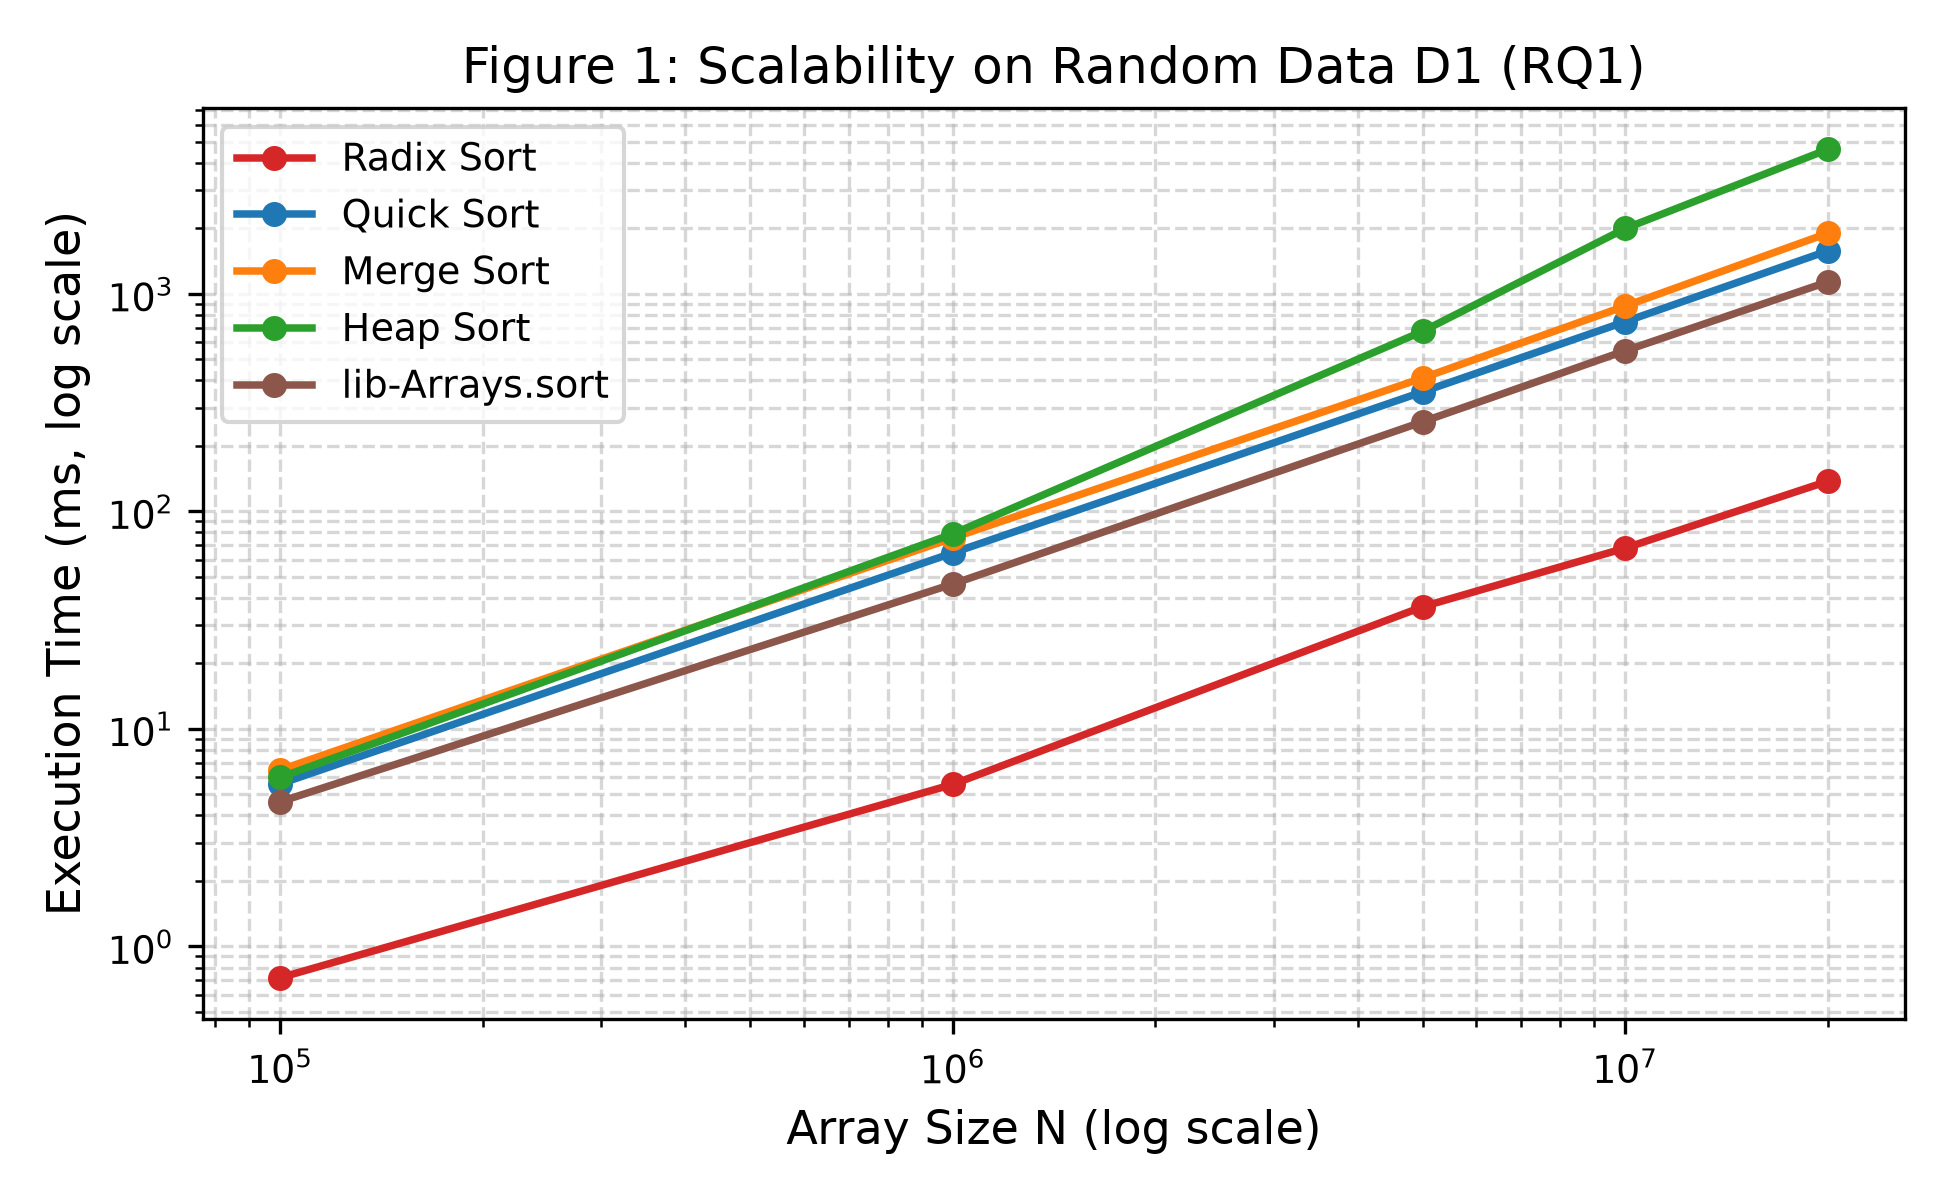
\includegraphics[width=\columnwidth]{fig1_rq1_scaling.png}
\caption{Quy luật tăng trưởng runtime theo kích thước $N$ từ $10^5$ đến $2\times 10^7$ trên thang Log-Log (RQ1, dữ liệu ngẫu nhiên $D_1$. Nguồn: \texttt{results/summary\_rq1.csv}).}
\label{fig:rq1}
\end{figure}

\textbf{Phân tích kết quả RQ1:}\\
1) \textbf{Sự thống trị của Radix Sort:} Radix Sort nhanh hơn Quick Sort gấp 11.5 lần và nhanh hơn Heap Sort gấp 33.5 lần tại $N = 2\times 10^7$. Điều này phản ánh rõ ưu thế vượt trội của độ phức tạp tuyến tính $O(4N)$ khi so với các thuật toán $O(N \log N)$.\\
2) \textbf{Sự suy giảm của Heap Sort do Cache Miss:} Mặc dù Heap Sort có cùng độ phức tạp lý thuyết $O(N \log N)$ như Quick Sort và Merge Sort, runtime thực tế của nó tăng vọt gấp 3 lần Quick Sort khi $N \ge 10^7$. Nguyên nhân cốt lõi là cấu trúc heap nhị phân phân bố dữ liệu theo bước nhảy cấp số nhân ($2i+1, 2i+2$), gây ra tỷ lệ cache miss rất cao khi kích thước mảng vượt quá dung lượng L3 cache.\\
3) \textbf{Bộ nhớ phụ:} Merge Sort và Radix Sort yêu cầu cấp phát đúng mảng phụ $N \times 4$ byte ($\approx 82$ MB tại $N=2\times 10^7$), trong khi Heap Sort duy trì bộ nhớ phụ tuyệt đối $O(1)$.

\subsection{RQ2: Tác động của tính thứ tự và độ trùng lặp khóa}
Bảng \ref{tab:rq2} tổng hợp thời gian thực thi trung vị và số thao tác cơ bản tại $N = 10^7$ trên 7 dạng dữ liệu ($D_1 \to D_5$).

\begin{table*}[t]
\caption{Thời gian thực thi trung vị (ms) và số thao tác tại $N = 10^7$ (RQ2. Nguồn: \texttt{results/summary\_all\_v2.csv}, script: \texttt{plot\_figures.py})}
\label{tab:rq2}
\centering
\footnotesize
\setlength{\tabcolsep}{4.5pt}
\begin{tabular*}{\textwidth}{@{\extracolsep{\fill}}lrrrrrr@{}}
\toprule
\textbf{Phân phối dữ liệu} & \textbf{Quick Sort} & \textbf{Merge Sort} & \textbf{Heap Sort} & \textbf{Radix Sort} & \textbf{pdqsort} & \textbf{Arrays.sort} \\
\midrule
$D_1$ (Ngẫu nhiên đều) & 938,7 ms & 1.107,7 ms & 1.782,4 ms & 113,8 ms & 992,6 ms & 713,7 ms \\
$D_2$ (Tăng dần) & 161,6 ms & 349,9 ms & 592,8 ms & 115,2 ms & \textbf{44,1 ms} & 2,2 ms \\
$D_3$ (Gần tăng dần) & 149,1 ms & 365,0 ms & 633,5 ms & 116,3 ms & 161,2 ms & 180,1 ms \\
$D_4$ (Giảm dần) & 157,9 ms & 403,0 ms & 686,2 ms & 116,7 ms & \textbf{54,5 ms} & 9,4 ms \\
$D_5$ ($K=10^3$) & 540,0 ms & 790,8 ms & 1.317,0 ms & 133,8 ms & 430,9 ms & 319,7 ms \\
$D_5$ ($K=10$)   & 331,8 ms & 544,9 ms & 604,6 ms & 144,0 ms & \textbf{147,4 ms} & 109,8 ms \\
$D_5$ ($K=2$)    & 261,7 ms & 396,6 ms & 319,3 ms & 150,0 ms & \textbf{46,4 ms} & 43,9 ms \\
\bottomrule
\end{tabular*}
\end{table*}

\begin{figure}[htbp]
\centering
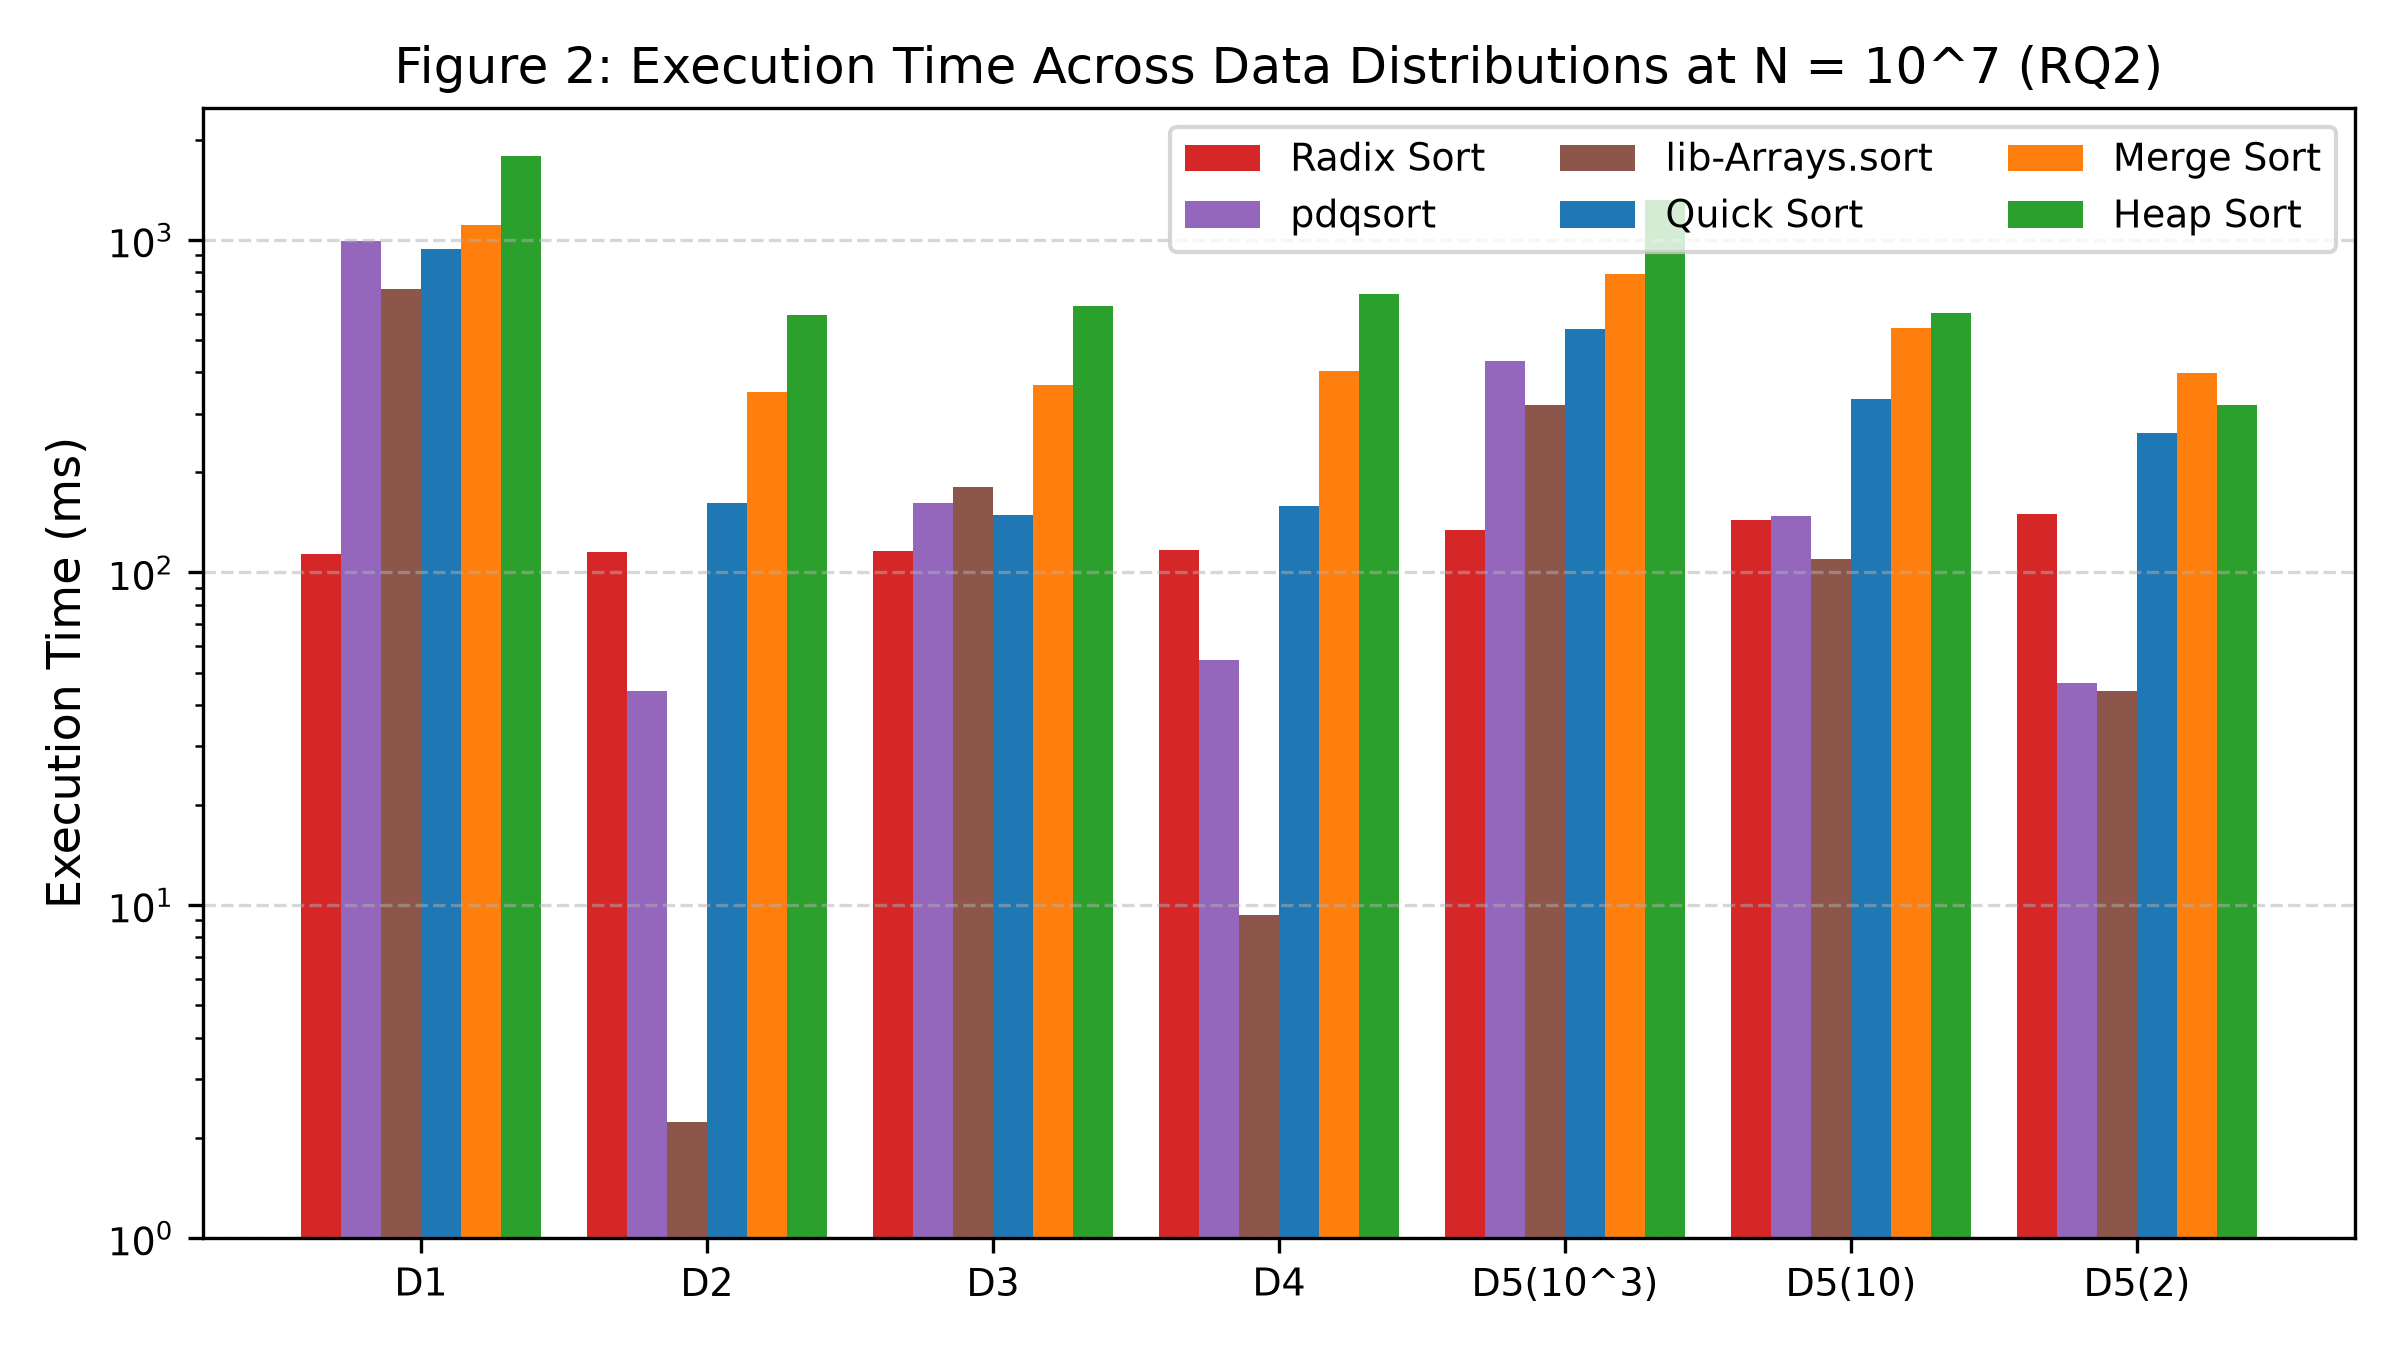
\includegraphics[width=\columnwidth]{fig2_rq2_runtime_by_distribution.png}
\caption{So sánh runtime của các thuật toán trên các phân phối dữ liệu khác nhau tại $N=10^7$ (RQ2. Nguồn: \texttt{results/summary\_all\_v2.csv} \& \texttt{results/rq3\_data.csv}).}
\label{fig:rq2_runtime}
\end{figure}

\begin{figure}[htbp]
\centering
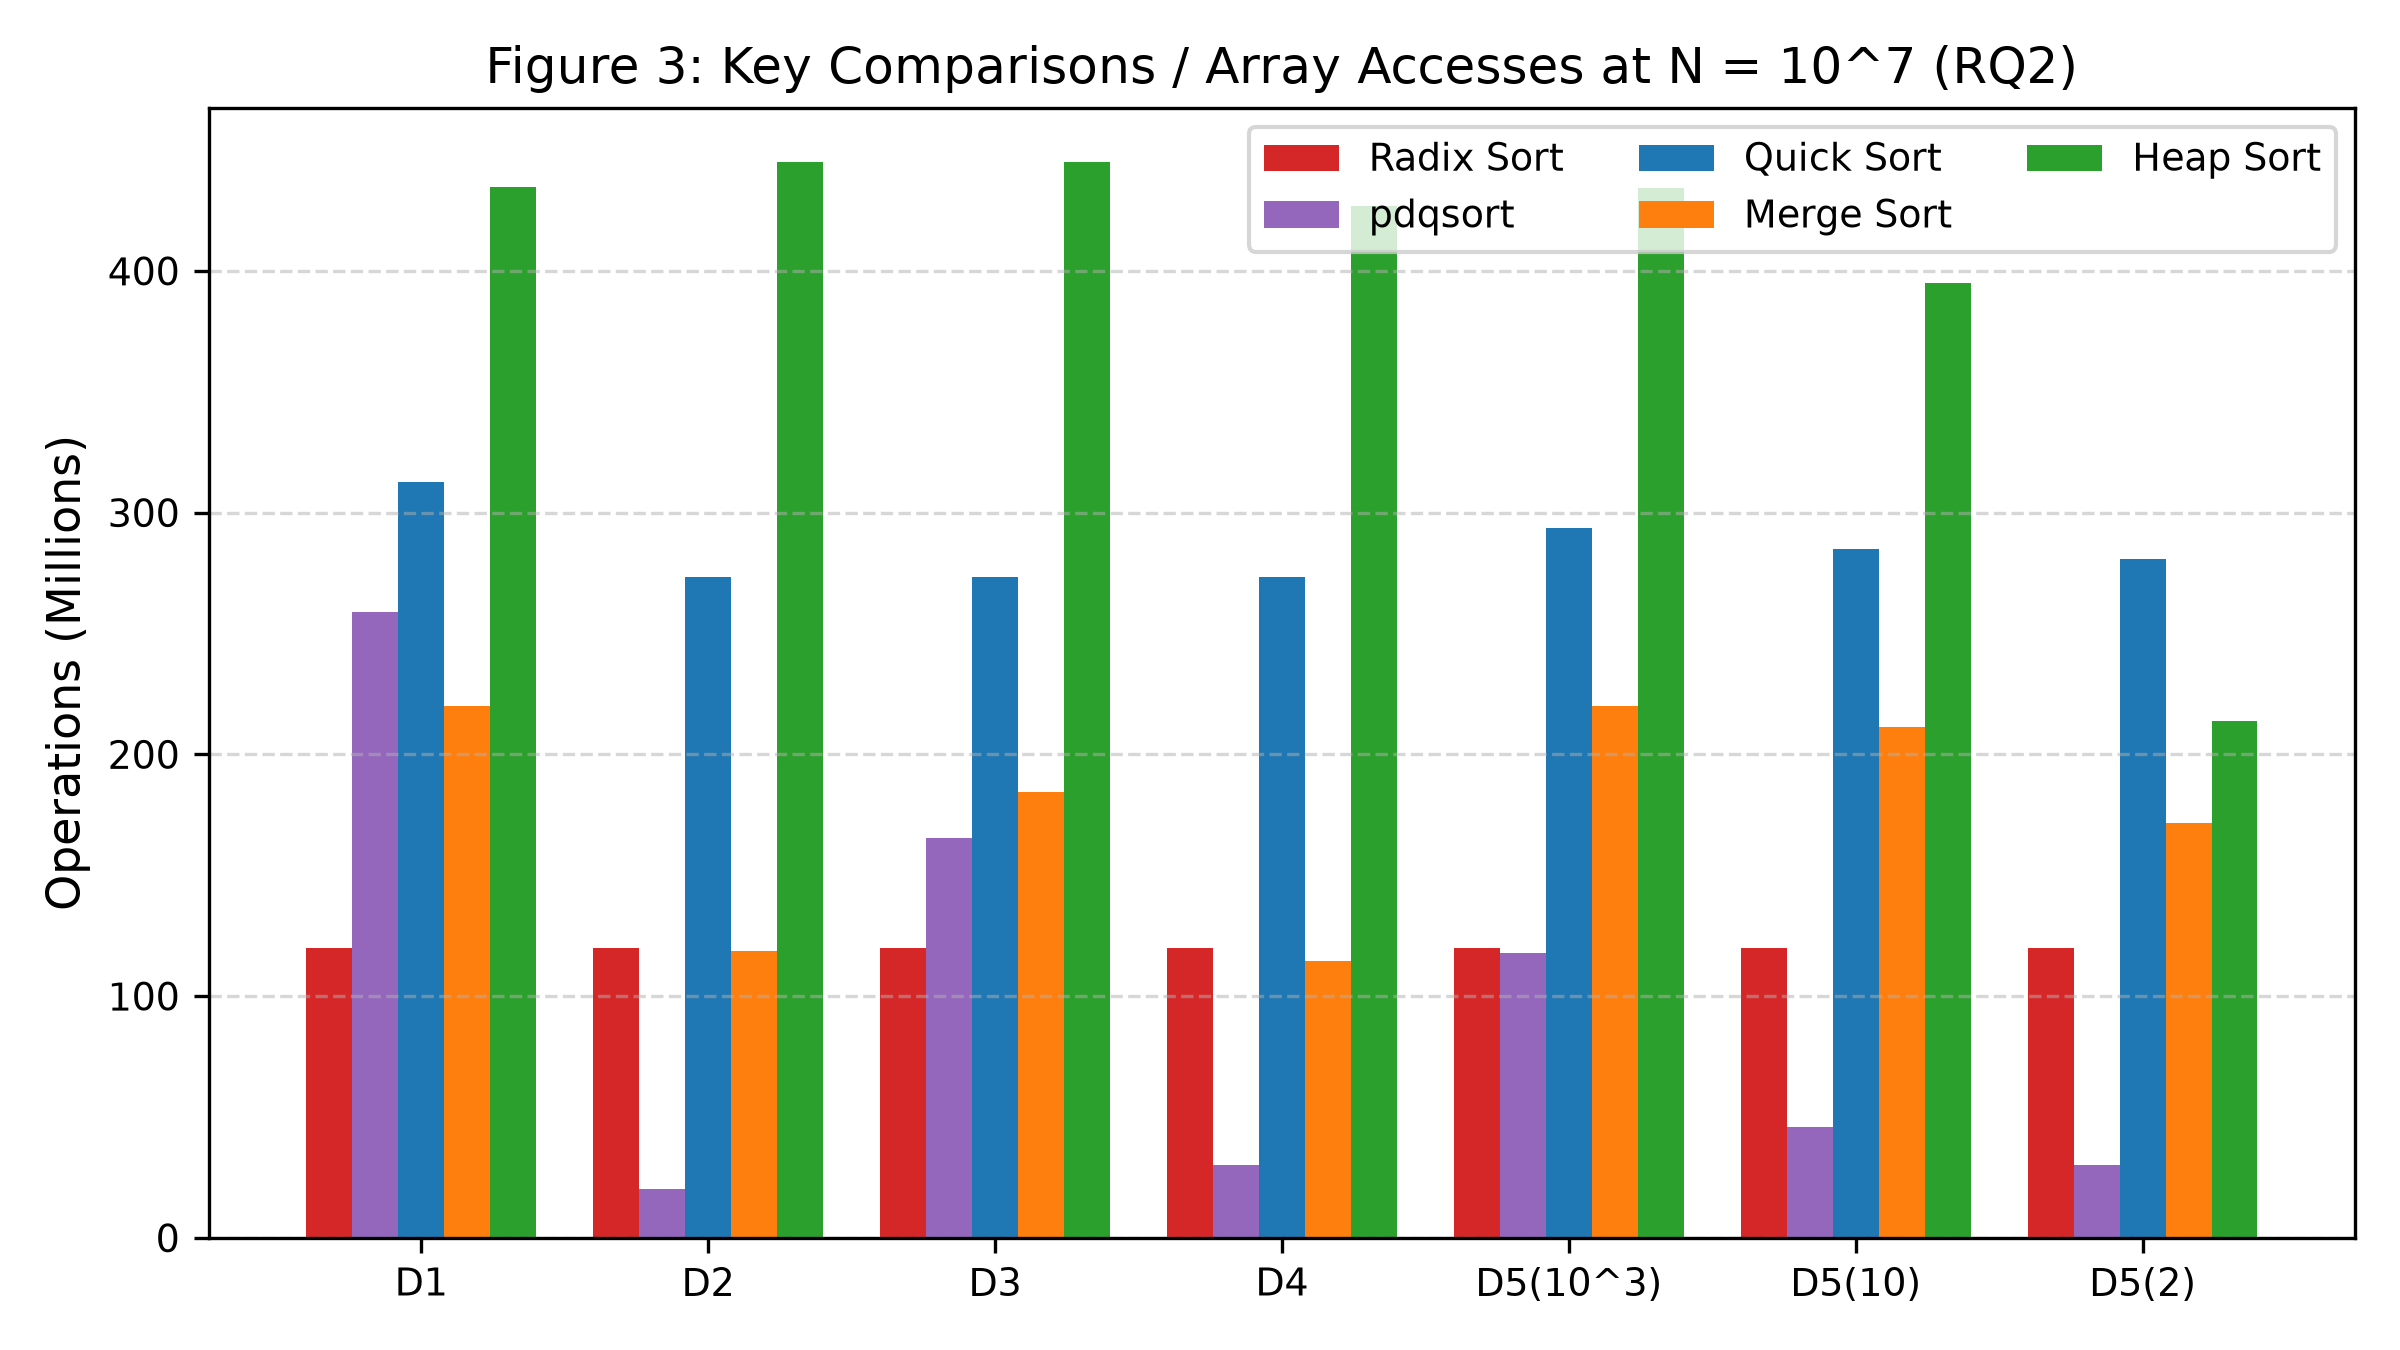
\includegraphics[width=\columnwidth]{fig3_rq2_ops_count.png}
\caption{Số lượng thao tác cơ bản tương ứng của các thuật toán trên các phân phối dữ liệu tại $N=10^7$ (RQ2).}
\label{fig:rq2_ops}
\end{figure}

\textbf{Phát hiện chính RQ2:}\\
- \textbf{Tính bất biến của Radix Sort:} Thời gian của Radix Sort dao động trong biên độ rất hẹp ($113 - 150$ ms) trên mọi phân phối đầu vào, do thuật toán luôn quét cố định đúng 4 lượt cơ số 256 và thực hiện đúng $12N$ ($1.2\times 10^8$) thao tác đọc/ghi ô nhớ.\\
- \textbf{Cơ chế phân hoạch Hoare trên dữ liệu trùng ($D_5$):} Quick Sort chạy nhanh hơn đáng kể trên $D_5$ ($K=2$ đạt 261.7 ms so với 938.7 ms trên $D_1$). Nguyên nhân là phân hoạch Hoare dừng hai con trỏ khi gặp phần tử bằng pivot, ép việc hoán đổi các khóa bằng nhau chia đều về hai phía, tạo ra cây đệ quy cân bằng hoàn hảo thay vì bị lệch một phía như phân hoạch Lomuto.\\
- \textbf{Heap Sort giảm thao tác trên $D_5$ ($K=2$):} Số phép so sánh của Heap Sort giảm mạnh từ 434 triệu ($D_1$) xuống còn 213 triệu ($D_5$ $K=2$), kéo thời gian giảm từ 1.782 ms xuống 319 ms. Hiện tượng này xuất hiện do lượng lớn nút có giá trị bằng nhau khiến điều kiện dừng \texttt{siftDown} được thỏa mãn ngay tại các tầng nông.

\subsection{RQ3: Hiệu năng pdqsort và thí nghiệm triệt tiêu (Ablation Study)}
Bảng \ref{tab:rq3} đối chiếu pdqsort đầy đủ với hai biến thể triệt tiêu \texttt{noA} (tắt phát hiện đoạn sắp) và \texttt{noB} (tắt gom khóa trùng) tại $N = 10^7$ từ các lượt benchmark độc lập.

\begin{table*}[t]
\caption{Đóng góp của Cơ chế A và B trong pdqsort tại $N = 10^7$ (RQ3. Nguồn: \texttt{results/rq3\_data.csv}, script: \texttt{plot\_figures.py})}
\label{tab:rq3}
\centering
\footnotesize
\setlength{\tabcolsep}{5pt}
\begin{tabular*}{\textwidth}{@{\extracolsep{\fill}}lrrrr@{}}
\toprule
\textbf{Phân phối dữ liệu} & \textbf{Quick Sort} & \textbf{pdqsort (full)} & \textbf{pdqsort (noA)} & \textbf{pdqsort (noB)} \\
\midrule
$D_1$ (Ngẫu nhiên đều) & 959,7 [952--968] & 992,6 [974--998] & 993,5 [987--1036] & 991,0 [970--1105] \\
$D_2$ (Tăng dần) & 143,6 [143,6] & \textbf{44,1} [44,1] & 314,6 [314,6] & 43,0 [43,0] \\
$D_3$ (Gần tăng dần) & 145,5 [144--160] & 161,2 [161--174] & 199,2 [199--200] & 160,6 [160--162] \\
$D_4$ (Giảm dần) & 149,9 [149,9] & \textbf{54,5} [54,5] & 333,1 [333,1] & 62,1 [62,1] \\
$D_5$ ($K=10^3$) & 570,4 [555--581] & 430,9 [424--443] & 428,4 [424--448] & 592,3 [565--598] \\
$D_5$ ($K=10$) & 352,3 [346--405] & \textbf{147,4} [145--151] & 144,1 [143--150] & 290,9 [287--306] \\
$D_5$ ($K=2$) & 279,4 [272--280] & \textbf{46,4} [45--56] & 45,4 [45--56] & 189,4 [189--190] \\
\bottomrule
\end{tabular*}
\vspace{1mm}\\
\raggedright \scriptsize \textit{Ghi chú: Đơn vị ms [min--max]. noA: tắt cơ chế presorted fast-path; noB: tắt cơ chế gom khóa trùng equal keys.}
\end{table*}

\begin{figure}[htbp]
\centering
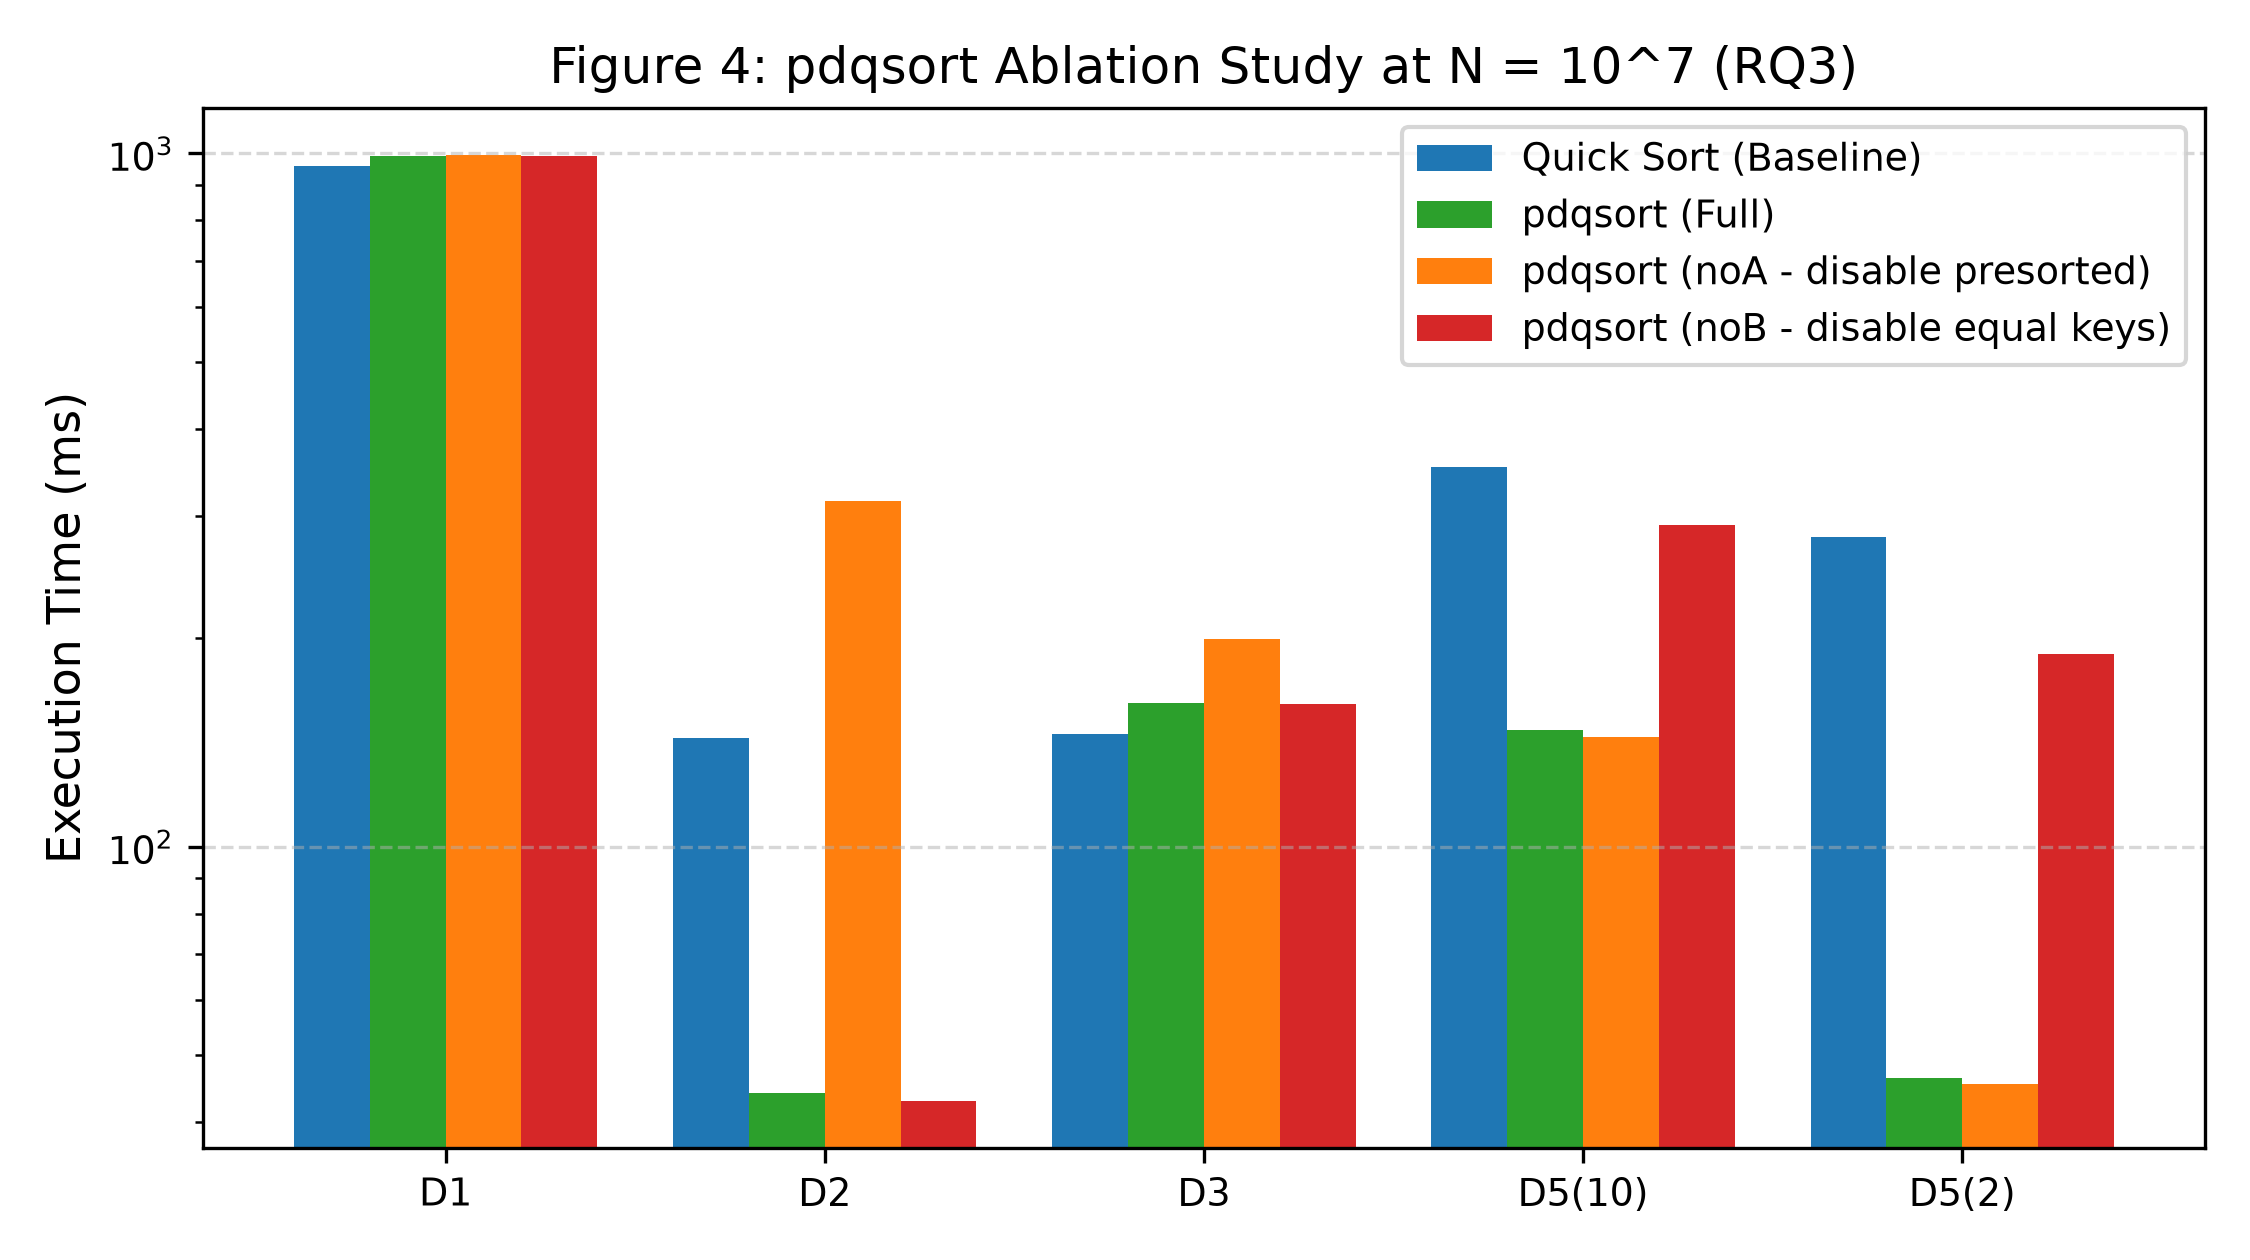
\includegraphics[width=\columnwidth]{fig4_rq3_pdq_ablation.png}
\caption{Ablation study bóc tách vai trò của Cơ chế A (\texttt{noA}) và Cơ chế B (\texttt{noB}) trong pdqsort tại $N=10^7$ (RQ3. Nguồn: \texttt{results/rq3\_data.csv}).}
\label{fig:rq3_ablation}
\end{figure}

\textbf{Phân tích định lượng đóng góp của từng cơ chế:}\\
1) \textbf{Vai trò của Cơ chế A trên $D_2, D_4$:} Trên mảng tăng dần $D_2$, pdqsort bản đầy đủ chỉ tốn $44,1$ ms. Khi tắt Cơ chế A (\texttt{noA}), runtime tăng vọt hơn 7 lần lên $314,6$ ms, đồng thời số phép so sánh tăng từ 20 triệu lên 202 triệu. Tương tự trên $D_4$, \texttt{noA} làm thời gian tăng từ 54,5 ms lên 333,1 ms. Điều này chứng minh partial insertion sort đã kích hoạt thành công fast-path tuyến tính $O(N)$ trên dữ liệu presorted.\\
2) \textbf{Vai trò của Cơ chế B trên $D_5$:} Trên mảng có mật độ trùng lặp cao ($K=2$), pdqsort bản đầy đủ hoàn thành trong $46,4$ ms. Khi tắt Cơ chế B (\texttt{noB}), thời gian tăng vọt hơn 4 lần lên $189,4$ ms, và số phép so sánh tăng từ 30 triệu lên 270 triệu. Việc gom các phần tử bằng pivot thông qua phân hoạch trái (\texttt{partitionLeft}) đã loại bỏ hoàn toàn đệ quy lặp lại trên các khóa trùng.\\
3) \textbf{Tính độc lập của hai cơ chế:} Trên $D_1$, cả ba phiên bản pdqsort ghi nhận thời gian gần như tương đương nhau ($\approx 991 - 993$ ms), chứng minh việc bổ sung hai cơ chế trên không gây overhead ngoài ý muốn trên dữ liệu ngẫu nhiên.

\subsection{Khảo sát mảng đối kháng (Killer Adversary Analysis)}
Để kiểm tra giới hạn chịu tải theo Mục 4 của đề tài, nhóm tiến hành thực nghiệm đối kháng bằng mảng hoán vị Musser \cite{musser1997introsort} đánh lừa trực diện phân hoạch Hoare và pivot median-of-three.

\begin{table}[htbp]
\caption{Đối chứng hiệu năng trên mảng đối kháng Killer Adversary}
\label{tab:killer}
\centering
\footnotesize
\setlength{\tabcolsep}{2.5pt}
\begin{tabular*}{\columnwidth}{@{\extracolsep{\fill}}lrrrr@{}}
\toprule
\textbf{Thuật toán} & $N$ & \textbf{Số phép so sánh} & \textbf{max\_depth} & \textbf{Trạng thái} \\
\midrule
Quick Sort & $2.000$ & $1.011.992$ & $1.000$ & Thoái hóa $O(N^2)$ \\
pdqsort & $2.000$ & \textbf{24.047} & \textbf{9} & An toàn $O(N \log N)$ \\
\midrule
Quick Sort & $10.000$ & $25.059.992$ & $5.000$ & Nguy cơ tràn stack \\
pdqsort & $10.000$ & \textbf{145.751} & \textbf{12} & Heap fallback \\
\bottomrule
\end{tabular*}
\end{table}

\textbf{Kết quả khảo sát đối kháng:}\\
- \textbf{Sự thoái hóa của Quick Sort giáo trình:} Trên mảng killer adversary $N = 2.000$, số phép so sánh của Quick Sort tăng vọt lên $1.011.992$ (tiệm cận mức cực đại $\approx N^2 / 4$), và độ sâu call stack đạt cực trị $1.000$ ($= N/2$). Khi mở rộng lên $N = 10.000$, số so sánh vọt lên 25 triệu và độ sâu là 5.000, đứng trước nguy cơ tràn call stack (\texttt{StackOverflowError}).\\
- \textbf{Cơ chế tự vệ của pdqsort:} Trên cùng dữ liệu đối kháng $N = 2.000$, pdqsort chỉ tốn $24.047$ phép so sánh (ít hơn 42 lần) và độ sâu chỉ là $9$. pdqsort phát hiện phân hoạch lệch nặng ($size < N/8$), kích hoạt hoán đổi phá mẫu (\texttt{breakPatterns}); khi số lần lệch vượt $\lfloor \log_2 N \rfloor$, thuật toán lập tức chuyển sang \texttt{HeapSort.sortRange}. Nhờ đó, pdqsort hoàn toàn miễn nhiễm trước các tấn công DoS bằng dữ liệu killer adversary.

% =========================================================================
% MỤC VI: ĐE DỌA TÍNH HỢP LỆ
% =========================================================================
\section{Đe dọa tính hợp lệ}
\begin{itemize}
    \item \textbf{Tối ưu hóa JIT và Garbage Collector:} JIT tier-4 compilation và các đợt dọn rác bất định của JVM có thể làm biến thiên kết quả. Nhóm kiểm soát bằng cách warmup 3--5 lượt và cưỡng bức \texttt{System.gc()} trước mỗi phép đo.
    \item \textbf{Giới hạn bộ nhớ Heap MXBean:} \texttt{MemoryPoolMXBean} chỉ phản ánh heap pool được JVM quản lý, không đại diện hoàn toàn cho tập làm việc bộ nhớ vật lý (RSS) ở tầng kernel hệ điều hành.
    \item \textbf{Phạm vi kiểu dữ liệu:} Kết luận thực nghiệm áp dụng cho số nguyên không âm 32-bit. Nếu mở rộng sang khóa 64-bit (\texttt{long}), Radix Sort sẽ cần 8 lượt cơ số 256, làm tăng gấp đôi chi phí và có thể làm thay đổi thứ hạng so với Quick Sort ở RQ1.
\end{itemize}

% =========================================================================
% MỤC VII: KẾT LUẬN VÀ KHUYẾN NGHỊ
% =========================================================================
\section{Kết luận và Khuyến nghị}
Qua khảo sát thực nghiệm quy mô lớn từ $10^5$ đến $2\times 10^7$ phần tử, nghiên cứu đưa ra các khuyến nghị có điều kiện:
1) \textbf{Radix Sort} là giải pháp tối ưu tuyệt đối về throughput thuần túy cho khóa số nguyên 32-bit trong các bài toán đối soát lớn, miễn là hệ thống chấp nhận chi phí mảng phụ $O(N)$.
2) \textbf{Heap Sort} là lựa chọn bắt buộc cho các hệ thống nhúng có tài nguyên hạn hẹp đòi hỏi bảo đảm nghiêm ngặt bộ nhớ phụ $O(1)$ in-place và runtime $O(N \log N)$.
3) \textbf{pdqsort} là thuật toán tổng quát ưu việt nhất cho thư viện chuẩn: duy trì tốc độ của Quick Sort trên dữ liệu ngẫu nhiên, đạt thời gian $O(N)$ trên dữ liệu presorted thông qua Cơ chế A, loại trừ suy thoái trên dữ liệu trùng qua Cơ chế B, và ngăn chặn triệt để nguy cơ thoái hóa $O(N^2)$ bằng cơ chế Introsort fallback.

\section*{Lời cảm ơn và Khai báo sử dụng AI}
Nhóm nghiên cứu tuyên bố có sử dụng các công cụ trí tuệ nhân tạo (AI Assistant) để hỗ trợ giải thích tài liệu lý thuyết, tối ưu cú pháp các kịch bản đo đạc và rà soát định dạng LaTeX chuẩn IEEE. Mọi số liệu thực nghiệm trong bài báo đều xuất phát 100\% từ các lượt chạy thực tế trên máy đo, được kiểm chứng chéo và lưu vết đầy đủ trong các tệp CSV của dự án.

% =========================================================================
% TÀI LIỆU THAM KHẢO
% =========================================================================
\begin{thebibliography}{00}
\bibitem{hoare1962quicksort} C. A. R. Hoare, ``Quicksort,'' \emph{The Computer Journal}, vol. 5, no. 1, pp. 10--16, 1962.
\bibitem{williams1964heapsort} J. W. J. Williams, ``Algorithm 232: Heapsort,'' \emph{Communications of the ACM}, vol. 7, no. 6, pp. 347--348, 1964.
\bibitem{bentley1993engineering} J. L. Bentley and M. D. McIlroy, ``Engineering a sort function,'' \emph{Software: Practice and Experience}, vol. 23, no. 11, pp. 1249--1265, 1993.
\bibitem{peters2021pdqsort} O. R. L. Peters, ``Pattern-defeating quicksort,'' arXiv preprint arXiv:2106.05123, 2021.
\bibitem{musser1997introsort} D. R. Musser, ``Introspective sorting and selection algorithms,'' \emph{Software: Practice and Experience}, vol. 27, no. 8, pp. 983--993, 1997.
\bibitem{mcilroy1999killer} M. D. McIlroy, ``A killer adversary for quicksort,'' \emph{Software: Practice and Experience}, vol. 29, no. 4, pp. 341--344, 1999.
\bibitem{sedgewick2011algorithms} R. Sedgewick and K. Wayne, \emph{Algorithms}, 4th ed. Boston, MA, USA: Addison-Wesley, 2011, \S2.2--2.4, \S5.1.
\end{thebibliography}

\end{document}
